\section{Related Work}

Nat�rlich sind wir nicht die Ersten, die mit einer Kombination aus realer und virtueller Welt experimentieren. Es gibt schon einige etablierte Spiele, die beides erfolgreich verbindet.
H�ufig wird es im Sinne von viralem Marketing zur Bewerbung eines neuen Produktes oder einer neuen Dienstleistung verwendet, ohne dieses direkt anzupreisen und ohne das Spiel als Werbeveranstaltung erkennen zu lassen.

\subsubsection{Ingress}
Auch Google selbst l�sst sich nicht lumpen und hat ein erfolgreiches Spiel implementiert. Ingress \cite{ingress} ist ein kooperatives interaktives Gesellschaftsspiel. 

\subsubsection{Pacman auf Google-maps}

Ein weiteres kleines Minispiel, welches sich Google hat einfallen lassen, lies sich nur eine bestimme Zeit lang spielen. Um den 1. April 2015 konnte man auf der normalen Google-Maps Seite die Stra�enkarte in ein Pacman-Spiel \cite{pacman} verwandeln und sich somit durch seine eigene Stadt mit dem kleinen gelben Kreis fressen.

\begin{figure}[htbp]
  \centering
    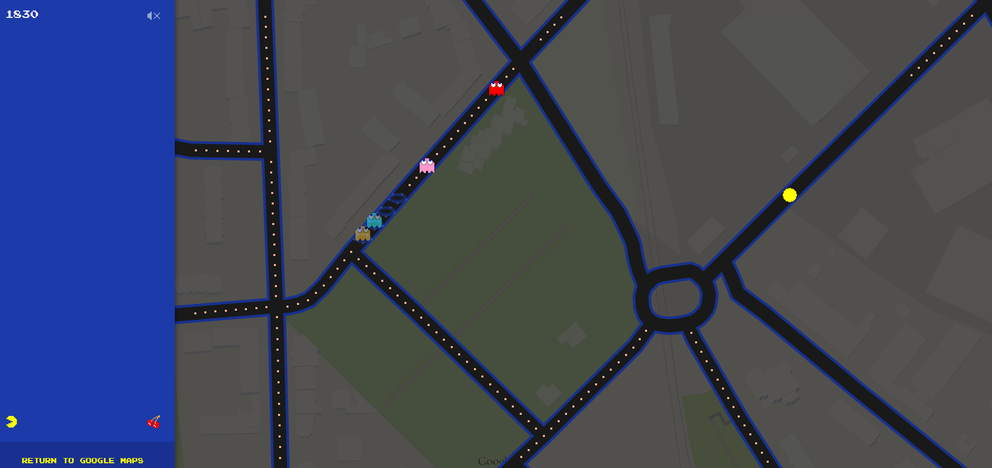
\includegraphics[width=0.9\textwidth]{2-Spielideen/2-3-Related_Work/pacman.png}
     \caption{Pacman auf Googlemaps}
\end{figure}


\subsubsection{Twinkomplex}

Eine �hnliche Idee hatte der Gr�nder von TwinKomplex. Er l�sst den Spieler in die Rolle eines Agenten schl�pfen und benutzt dazu Google-Maps und andere Open-Source Daten. So m�ssen die Agenten von einen Schnipsel zum anderen finden. \cite{twinkomplex}